\chapter{Modelo de datos}
\label{cap:modelo}
En este capitulo se mostrará el diseño de datos lógico y físico generado para el proyecto que estamos presentando, correspondiente a la reestructuración del sistema actual. 

\section{Modelo de datos lógico}
\begin{figure}[htb]
  \begin{center}
    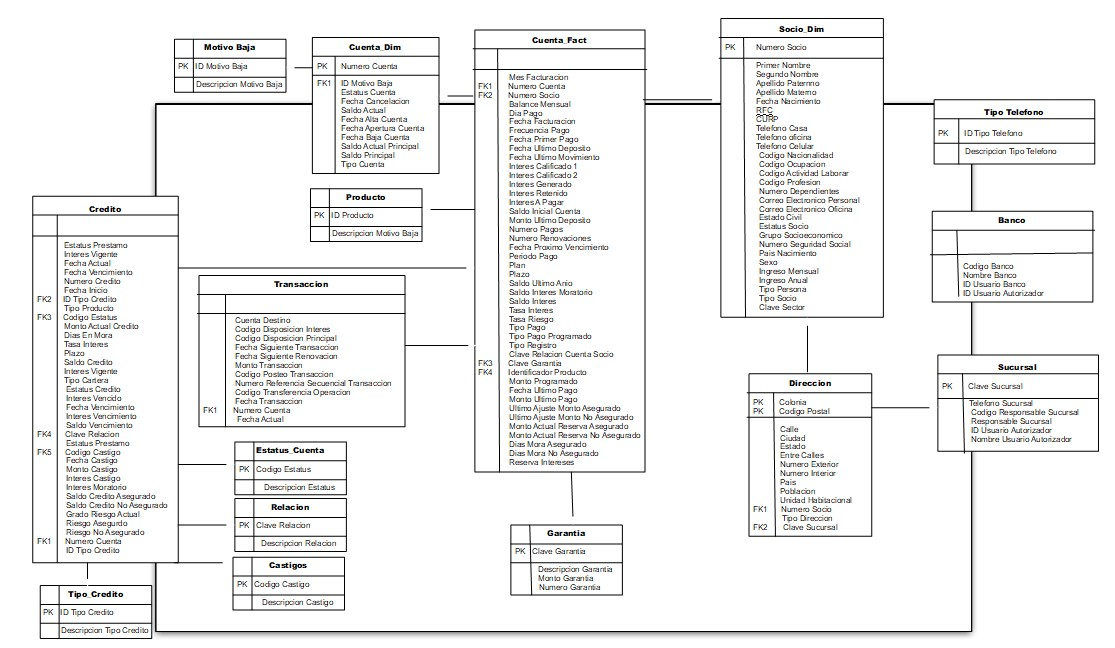
\includegraphics[width=\linewidth]{Modelo_logico.jpg}
        \caption{Modelo logico de la base de datos.}
    \label{fig:modelo-logico}
  \end{center}
\end{figure}


\section{Modelo de datos físico}

\cleardoublepage

%%% Local Variables:
%%% TeX-master: "Tesis"
%%% End:
